This section describes the various electronic components used in the project, as
well as their interface to one another.  This section focuses on the hardware
and electrical aspect of the components; one should refer to Section
\ref{embeddedSoftwareAutomation} for details regarding the software
implementation.  

\subsection{Hardware Components}
The following components were attached to an Atmel AT90 microcontroller either directly, or indirectly through a breadboard.  

\subsubsection{Atmel Microcontroller}
The Hovercraft project is centered around the AT90USB1287 processor from Atmel, mounted on a AT90USBKey which is shown in Figure \ref{fig:at90usbkey}.

\begin{minipage}{6.5in}
  \centering
    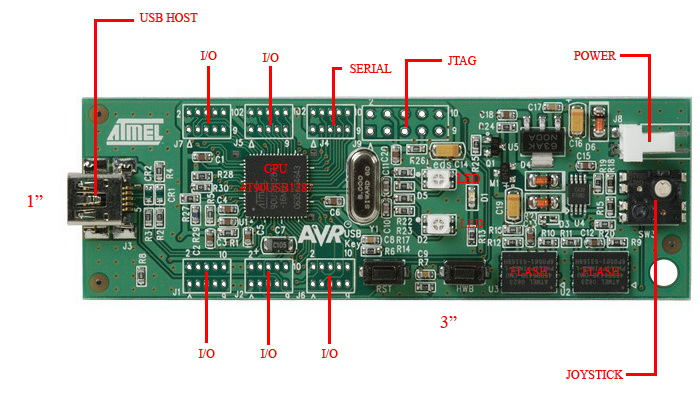
\includegraphics[width=110mm]{imageSources/at90usbkey.png}
  
  \captionof{figure}{Atmel AT90USBkey} 
  \label{fig:at90usbkey}
\end{minipage}
\vspace{0.1in}

Some of the most notable features of this board include:
\begin{itemize}
\item USB Interface
\item 4+1-ways joystick
\item 2 Bi-Color LEDs
\item temperature sensor
\item serial dataflash memories
\item On-board RESET button 
\item On-board HWB button to force bootloader section execution at reset.
\item System clock: 8 MHz crystal
\end{itemize}

\subsubsection{Radio}
The radio used for hovercraft-basestation and hovercraft-hovercraft communication is the TRW-24G.  The datasheet for this component can be found online\footnote{www.kosmodrom.com.ua/data/TRW-2.4G.pdf}.  The radio operates at a frequency of 2.4 to 2.527 GHz and has a working voltage of 3 Volts (ranging from 1.8 to 3.6 Volts).  The radio can transmit anywhere from 250 Kbps to 1000 Kbps (1Mbps).  Communication is segmented into 128 distinct channels which each occupy a 1 MHs chunk of spectrum. In figure \ref{radioFig}
the radio has pins all clustered together. The radio is also able to have a connector attached to the pins that will make it compatible with a traditional bread board. This connector changes the clustered pins into 10 pins in a row.

\begin{minipage}{6.5in}
  \centering
    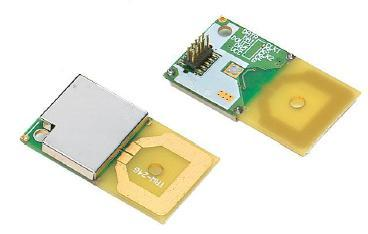
\includegraphics[width=110mm]{imageSources/radio.png}
  
  \captionof{figure}{TRM-24G RF 2-way Radio} 
  \label{radioFig}
\end{minipage}

\subsubsection{Motors}
Several types of motors, as well as other supporting circuitry, are required to propel and maneuver the hovercraft. \\ 

\noindent{\bf The DC Motor}\\

Figure \ref{hBridge} is an image of the L393D H-Bridge which is the H-bridge used for this project.  This chip has the ability to run two H-bridges. 


\begin{minipage}{6.5in}
 \centering
    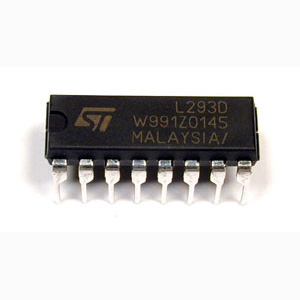
\includegraphics[width=70mm]{imageSources/hBridge.png}
    \captionof{figure}{L2930 H-Bridge} 
  \label{hBridge}
\end{minipage}
\vspace{0.1in}


The L293D chip contains four input/output channels that can be used for two bridges. Each bridge (i.e. two channels) contains an enable connection required to operate it. If the enable connection is given HIGH input, channel output is the same as channel input. If the enable is not connected or given LOW input, the channel output will be high impedance. The L293D chip requires two connections at all times: a supply voltage (+5V) and ground (+0V). The chip also provides a second logic supply voltage if lower voltage operation is required.

The 74HC04 hex inverter chip is very simple. If the chip receives a HIGH signal, it will return a LOW signal, and visa versa. This hex inverter provides six input/output combinations. The inverter requires 5V of power and to be grounded.

\begin{minipage}{6.5in}
  \centering
    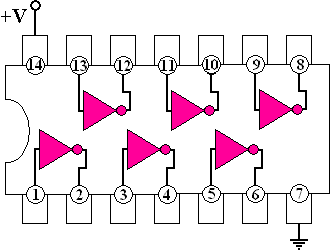
\includegraphics[width=70mm]{imageSources/hexInverter.png}
 
  \captionof{figure}{74HC04 Hex Inverter} 
  \label{hexInverter}
\end{minipage}
\vspace{0.1in}

\noindent {\bf The Servo Motor}\\

The servo used is the Hitec HS-55(See figure \ref{servo}). This is a very small servo that is controlled using pulse width control. It requires at least 4.8 volts of power, so it must be powered by the source, the AT90 only produces 3.3 volts.

\begin{minipage}{7in}
  \centering
    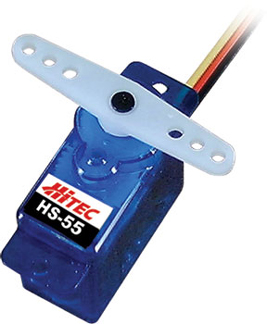
\includegraphics[width=70mm]{imageSources/servo.png}
  
  \captionof{figure}{Hitec HS-55 Servo} 
  \label{servo}
\end{minipage}
\vspace{0.1in}

\subsubsection{Joystick}
 A modified serial joystick is used to control the hovercraft. The joystick has a connector that is the male counter part of the connector shown in figure \ref{joystick}. A female port that had its underside exposed is  wired so that the X, Y ground and power are easily connected to the AT90 board or the bread board. 

\begin{minipage}{7in}
  \centering
    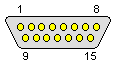
\includegraphics[width=90mm]{imageSources/joystick.png}
  
  \captionof{figure}{Joystick Pinout} 
  \label{joystick}
\end{minipage}
\vspace{0.1in}

\begin{minipage}{7in}
Table \ref{joystickPinout} describes the functions of each pin of the joystick.

\captionof{table}{The joystick pinout}
\centering
\begin{tabular}{ c c c } 
  Pin Number & Signal Name & Description \\
  \hline
 1 & +5V & Power \\
 2 & Right Button 1 & Button 1 \\
 3 & X-Position 1 & Joystick 1 X-Coordinate \\
 4 & Signal GND & Ground \\
 5 & Signal GND & Ground \\
 6 & Y-Position 1 & Joystick 1 Y-Coordinate \\
 7 & Left Button 1 & Button 2 \\
 8 & +5V & Power \\
 9 & +5V & Power \\
 10 & Right Button 2 & Button 4/Joystick 2 Right button \\
 11 & X-Position 2 & Joystick 2 X-Coordinate \\
 12 & MIDI Out & MIDI Output \\
 13 & Y-Position 2 & Joystick 2 Y-Coordinate \\
 14 & Left Button 2 & Button 3/Joystick 2 Left button \\
 15 & MIDI In & MIDI Input \\
\end{tabular}
\label{joystickPinout}

\end{minipage}
\vspace{0.1in}

\subsubsection{UART}
For testing purposes, the ability to have two UART readings was beneficial. The serial UART connection is connected to a windows machine. For serial UART connections, the ADM33L chip is used to convert the signal. This chip is intended for use with transmitting and receiving devices. In this project, it is used for RS-232 transmission of data from the AT90 to a serial connection on a HyperTerminal running on the computer. This chip has an on board voltage converter to allow it to run from a single 5 volt power supply. 
\begin{minipage}{6.5in}
  \centering
    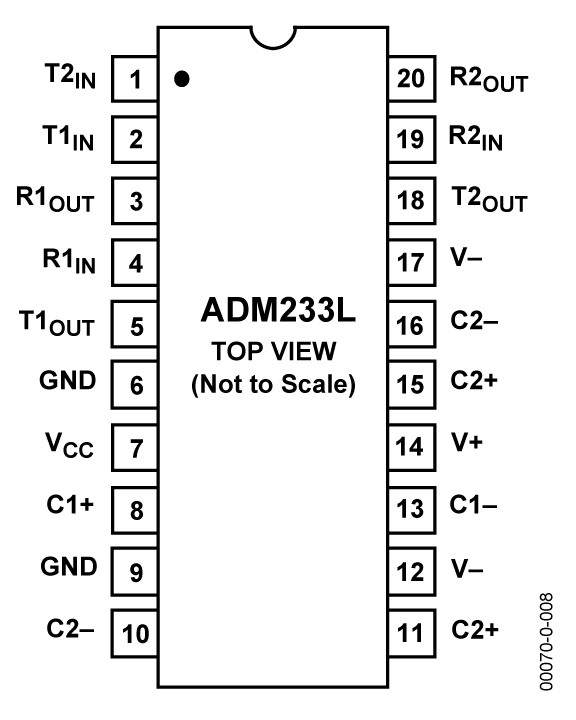
\includegraphics[width=90mm]{imageSources/serialUART.png}
  
  \captionof{figure}{Serial UART Schematic} 
  \label{serialUART}
\end{minipage}

The prefered method of communication with an external computer is through the use of a USB to UART Bridge - FT232RL\footnote{www.ftdichip.com/Documents/DataSheets/DS\_FT232R.pdf }. This bridge is able to be connected directly to the board with out the use of an extra chip. This chip is powered using the 3.3 volts of power provided by the connection to the computer. Figure \ref{usbUART} is a picture of this chip mounted with pins. 

\begin{minipage}{6.5in}
  \centering
    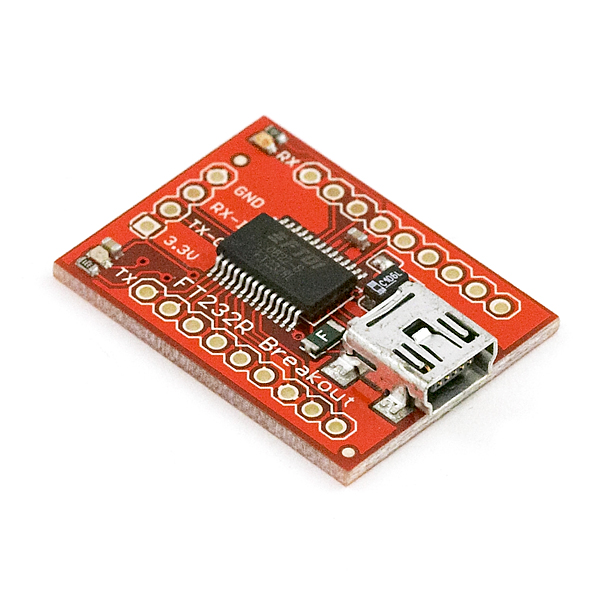
\includegraphics[width=90mm, height= 70mm]{imageSources/usbUART.png}
  
  \captionof{figure}{USB UART} 
  \label{usbUART}
\end{minipage}


\subsubsection{Sonar}
 The sonar used in this project is the MaxSonar EZ1\footnote{www.maxbotix.com/uploads/LV-MaxSonar-EZ1-Datasheet.pdf} depicted in figure \ref{sonar}. This sonar is capable of both long and short distance readings. It can tell if there is an object present from 0-254 inches, and gives distance information for objects within 6 to 254 inches. This sonar has ground, VCC, enable and three different pins to read information(PWM, analog, digital). The PWM signal is easily read with use of one of the AT90 input capture registers and is the method used in this project.  When the enable pin is pulled high the sonar will omit a pulse. Information regarding pulse distance is then transfered to the board through the RX pin. 

\begin{minipage}{6.5in}
  \centering
    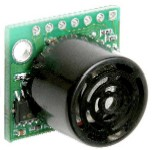
\includegraphics[width=70mm, height= 70mm]{imageSources/sonar.png}

  \captionof{figure}{Max Sonar EZ1} 
  \label{sonar}
\end{minipage}
\vspace{0.1in}

\subsection{Connections and Interface Design}
This section describes the connections among the various components, as well as other factors relating to the design of the electronic configurations used.  

\subsubsection{Power}
To power many of the components (Motors, Sonar, RS-232 Uart)  more than the 3.3 volts of power than the USB provided is required. These components can be powered by battery or a power cord from the wall. The batteries that are used for this project produce 7 volts and the direct power from the wall reads between 9-12 Volts (Specifications indicate that the cords produce 12, but they often had fluctuating readings).  Both sources of power need to be minimized to a managable 5 volts.  Figure \ref{power12to5} shows the setup to do this conversion.

\begin{minipage}{6.5in}
  \centering
    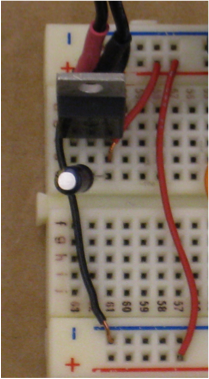
\includegraphics[height = 4in]{imageSources/power12to5.png}
  
  \captionof{figure}{Conversion from 12 to 5 volts} 
  \label{power12to5}
\end{minipage}

\subsubsection{Radio Connections}
 Each of the boards has one radio attached for communication. The leader hovercraft uses the radio to send information regarding motor movement to the follower, as well as information to the base station regarding the status of the hovercraft.  The radio on base station sends an initiate message to the leader and receives information to display via uart. The follower hovercraft receives information from the leader so that it is able to follow.

All of the wires from the radio go to port E. The Radio ground pin must also be connected to the ground on the bread board. The pin assignments for the required pins from the radio are modeled in figure \ref{radioConnect}.

\begin{minipage}{6.5in}
  \centering

    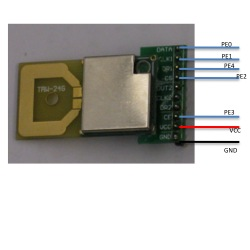
\includegraphics[width=90mm]{imageSources/radioConnect.png}
  
  \captionof{figure}{Radio Wiring Layout} 
  \label{radioConnect}
\end{minipage}

\subsubsection{Motor Connections}
An H-bridge is used to  control a motor that is required to spin in two different directions. Figure \ref{hBridgeConnect1} a diagram behind the theory of an H-Bridge\cite{hbridgewiki}. An h-bridge is composed of a power source, four switches and a motor. The switches can all be in one of two positions, open or closed. There are only two different positions that the entire h-bridge can be in (shown in the diagram below). On the left, the lower left and upper right switches are open. this makes a circuit that goes through the motor from left to right, this will make the motor spin one way.  In the right diagram the other two switches are open, this makes the current flow through the motor from right to left, making the motor spin in the opposite direction.

\begin{minipage}{6.5in}
  \centering
    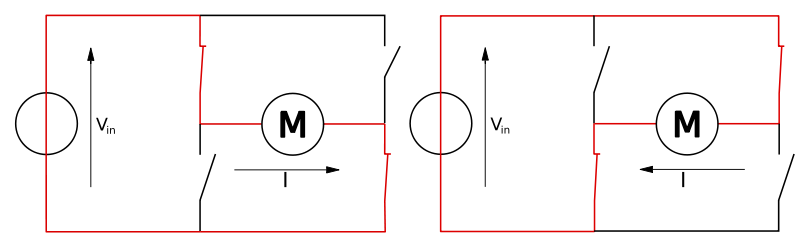
\includegraphics[width=90mm]{imageSources/hBridgeConnect1.png}
  
  \captionof{figure}{Diagram of the H-bridge for a DC Motor} 
  \label{hBridgeConnect1}
\end{minipage}


\begin{minipage}{6.5in}
  \centering
    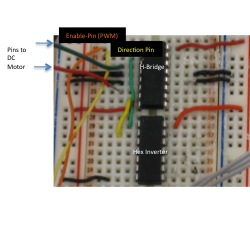
\includegraphics[width=90mm]{imageSources/hBridgeConnect2.png}
  
  \captionof{figure}{Layout of the H-bridge} 
  \label{hBridgeConnect2}
\end{minipage}
\vspace{0.1in}

In figure \ref{hBridgeConnect2}, the orange enable pin is attached to the output compare register OCR0A on the AT90. This pin outputs the PWM signal needed to control the speed of the motor.  The direction of the motors is controlled through  yellow direction pin. This pin is connected to pin C1 on the AT90. This pin is either pulled HIGH or LOW. The value from this pin is also pulled through the inverter and connected to the other input pin with the H-bridge. This change in values changes the position of the switches in the H-bridge.

\subsubsection{Joystick Connections}

In phase one and two of the project, a joystick is used to move the hovercraft and test maneuverability. The joystick used is a modified analog joystick. The joystick's wiring is modified to change how the potentiometers are read. Details of how the conversion from analog to digital are outlined in section \ref{sec:JoystickConst}.


Figure \ref{joystickConnect} outlines the connections between the joystick at the AT90.  Pin 3, 6 and 13 on the connector for the joystick are values x, y1 and y1 respectively. These connections are connected to port F on the AT90 in pins 1, 2 and 4.


\begin{minipage}{6.5in}
  \centering
    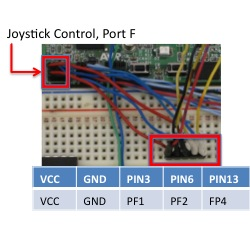
\includegraphics[width=70mm]{imageSources/joystickConnect.png}
  
  \captionof{figure}{Joystick Connection: Pin Layout} 
  \label{joystickConnect}
\end{minipage}
\vspace{0.1in}

\subsubsection{UART Connections}


The ADM233L connects to both the serial cable, and the AT90. The diagrams for the two components are outlined in figure \ref{Uart1} Figure \ref{uartConnect1} is a diagram of the ADM233L and the connections to the AT90 and the serial connector while figure \ref{uartConnect2} outlines how the serial cable connector side of the connections. 
 
\begin{figure}[htp]
  \begin{center}
    \subfloat[UART Pin Layout for ADM233L]{\label{uartConnect1}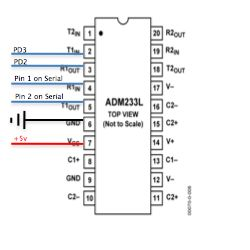
\includegraphics[width=0.4\textwidth]{imageSources/uartConnect1.png}}
    \subfloat[UART Pin Layout For Serial]{  \label{uartConnect2} 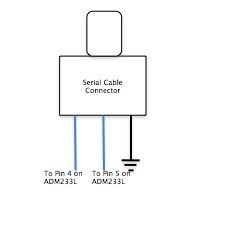
\includegraphics[width=0.4\textwidth]{imageSources/uartConnect2.png}}
  \end{center}
 \caption{Pin Diagrams for UART serial connections}
 \label{Uart1}
\end{figure}


Figure \ref{uartConnect3} depicts the the UART layout of the board. In this picture, the layout of the power supply is also visible. 

\begin{minipage}{6in}
  \centering
   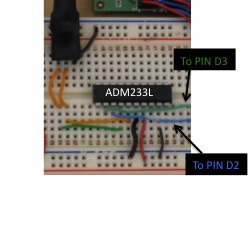
\includegraphics[width=0.6\textwidth]{imageSources/uartConnect3.png}
  
  \captionof{figure}{UART Wiring Layout} 
  \label{uartConnect3}
\end{minipage}
\vspace{0.1in}


USB UART is connected to the AT90 trough use of the same pins as the serial UART.  This USB UART chip has three output wires.  GND, TX-O, RX- I and is connected directly to the AT90 using port D. TX-O connects to PD2 and TX-I connects to PD3, the GND output connects directly to ground on the AT90.

\subsubsection{Servo Connections}
The servo motor requires 5 volts of power, to be connected to ground and a pwm signal to run. To generate the PWM signal a 16 bit timer must be enabled and the input wire on the servo must be connected to the proper output compare. For this component we used timer 1 and connected the servo to OC.1B which is located on PB6.

\subsubsection{Sonar Connections}
The sonar must be connected to two pins on the AT90 and to ground and power on the bread board. We decided to calculate the distance using PWM even though we could have used a few methods. (See sonar implementation for details on the conversion.)  For this the sonar needed to be attached to a pin on the board to be triggered when the input goes high. This pin also needs to be associated with a timer. We chose to use timer three for our sonar, and Input Capture Register (ICP3) to read the input which is located on port C7. The sonar will also only fire when the RX pin reads high. So we connected the RX pin to PC6 and then set that pin either high or low.

\begin{minipage}{6.5in}
  \centering
    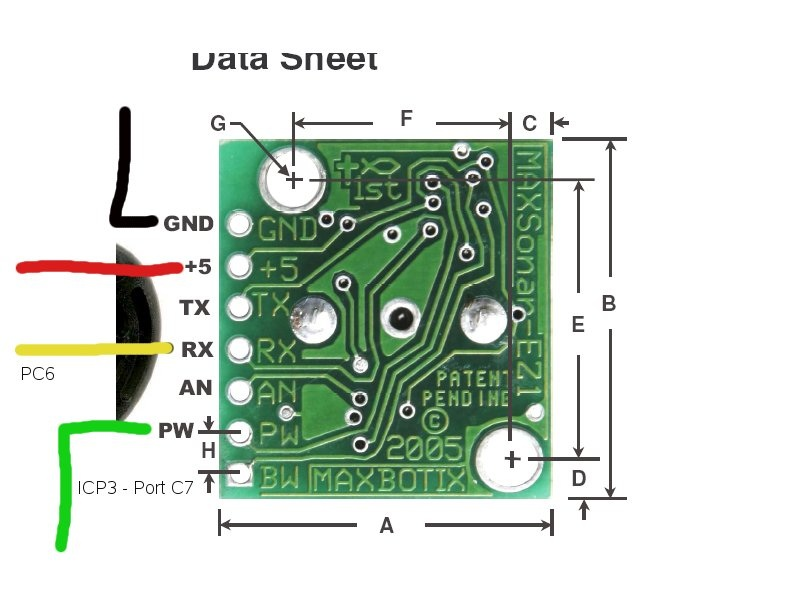
\includegraphics[width=90mm]{imageSources/sonarConnect.png}
 
  \captionof{figure}{Sonar Wiring Layout} 
  \label{sonarConnect}
\end{minipage}
